% !TEX root = ../thesis-example.tex
%
\chapter{A Bayesian Quasi-Randomized neural network, and its application to the optimization of black box functions}
\label{sec:bayesian_rvfl}

\section{Introduction}
\label{intro}

In this chapter, we present a Bayesian Quasi-Random Vector Functional Link (BQRVFL) neural network model, with one hidden layer. It is a hybrid penalized regression/neural networks model on an augmented data set. In this hybrid regression model, we assume that the regression parameters are governed by a prior distribution, and that the hidden layer's nodes are (quasi-)randomized. As a prior distribution for the regression parameters, we will use a multivariate Gaussian distribution. And for the simulation of the nodes in the hidden layer, we will use a Sobol sequence. 

\medskip

To the best of our knowledge, randomized neural networks were introduced by \cite{schmidt1992feedforward}, and the Random Vector Functional Link neural networks (RVFL) were introduced by \cite{pao1994learning}. RVFL networks are \textit{multilayer feedforward} neural networks, in which there is a \textit{direct link} between the predictors and the output variable, aiming at capturing the linear relationships. And in addition to the \textit{direct link}, there are new features, the hidden nodes (the dataset is augmented).

\medskip

The RVFL networks have been successfully applied to solving different types of classification and regression problems; see for example \cite{dehuri2010comprehensive}. Here, we will use RVFL networks with only one hidden layer.

\medskip

With the BQRVFL model presented here, it is possible to obtain predictions from a nonlinear model (actually, a combination of a linear and a nonlinear model), along with confidence intervals around the model's predictions. The choice of this relatively simple Gaussian prior should not, however, prevent the user from checking the confidence intervals around the predictions. 

\medskip 

There are other types of models, which are also capable of achieving this purpose - obtain predictions from a nonlinear model, along with confidence intervals around the model's predictions - like Gaussian process regression models (cite Rasmussen et al. (2006)) and random forests models with confidence intervals (cite Wager et al. (2014)). Depending on the problem at hand, and the desire from the user for a higher  accuracy and/or interpretability, one of these alternative models could also be considered.    

\medskip 

In section \ref{sec:modelprez}, we present the BQRFVL model, with one hidden layer. Formulas for the estimation of its parameters are given, along with formulas for the calculation of confidence intervals around the predictions. The model's predictions on a validation set, and on simulated data from (cite Sapp (2014)) are also presented. 

\medskip 

In section \ref{sec:bayesopt}, the model is used as a workhorse for Bayesian optimization (cite Mockus et al. (1978)). This type of optimization methods are useful for finding minima or maxima of black box functions, whose evaluations are expensive, and gradients are not necessarily available in a closed form. It has been shown to be very effective on challenging optimization functions (cite Jones (1998) and Snoek et al. (2015)).

\medskip 

The idea of Bayesian optimization is to optimize an alternative, cheaper function called the acquisition function, rather than the main, expensive objective function. For doing this, the uncertainty around the predictions of an alternative machine learning model - called the surrogate model - is used in a way that will be described in more details in section \ref{sec:bayesopt}. 

\medskip 

The surrogate model's posterior distribution tries to approximate the objective function in the best way. And this posterior distribution is enhanced, as more points of the objective function are evaluated. Gaussian process regression models are often used are surrogate models (cite Snoek et al. (2015) for example). Here, the surrogate model will be the BQRVFL model presented in \ref{sec:modelprez}.

\medskip 

We apply Bayesian optimization, using the BQRVFL model, to the minimization of the cross-validation error (produced on discount curve forecasting) of four machine learning models. One of these models is based on an RVFL applied to multivariate time series forecast (cite Moudiki et al. (2018)). The second one applies Kernel Regularized Least Squares (cite chapter) (KRLS hereafter) directly to the curves' observation dates and time to maturities. The two remaining models are based on the popular DNS framework, and are a DNS-KRLS and a DNS-RVFL (more details here or refer to another section). 

\newpage

\section{Description of the model}
\label{sec:modelprez}

\subsection{Estimation of the parameters and confidence intervals}

We consider a response variable $y \in \RR^n$ that has to be explained as a function of $p$ predictors stored in a matrix $\textbf{X} \in \RR^{n \times p}$. The data set $\textbf{X}$ is augmented by a set of new predictors: 
$$
g \left(\textbf{X} W \right)
$$
where $g$ is an activation function, as in of neural networks models, and $W \in \RR^{p \times L}$ are the nodes in the hidden layer, obtained from a deterministic sobol sequence of quasi-random numbers (cite Niderreiter (1992) and Boyle et Tan (1997)). $L$ is the number of nodes in the hidden layer. 

\medskip 

The parameters $W$ are used to combine the $p$ columns of \textbf{X} into $L$ new variables, hence taking into account the potential nonlinear relationships between the response $y$ and the predictors $\textbf{X}$ when passed through the activation function $g$. Having obtained a new set of predictors stored in columns in a matrix $\textbf{Z} = \left[ \textbf{X} \:\:  g \left(\textbf{X}W\right)\right]$, we apply a Bayesian linear regression model, to explain $y$ as a function $\textbf{Z} \beta$ of the new $p + L$ predictors. We assume that $y$ could be explained as: 
$$
y = \textbf{Z} \beta + \epsilon
$$
where $\beta \sim \MN(0_{\RR^{p + L}}, I_{p + L})$ are the parameters of the model that have to be estimated,  and $\epsilon \sim \MN(0_{\RR^n}, \sigma^2 I_n)$ is the error term. It is possible to show, in a Bayesian linear regression setting (cite Rasmussen et al. (2006) for example, for details) that for new observations arriving in the model and stored in matrix $\textbf{Z}_*$ , we have the following properties for the associated predictions: 
$$
y* \sim  \MN(\textbf{Z}_* \mu_{\beta | y, \textbf{Z}}, \: \textbf{Z}_* \Sigma_{\beta | y, \textbf{Z}} \textbf{Z}_*^T + \sigma^2 I_n)
$$
with 
$$
\mu_{\beta | y, \textbf{Z}} = \textbf{Z}^T \left( \textbf{Z} \textbf{Z}^T + \sigma^2 I_n\right)^{-1}y
$$
and 
$$
\Sigma_{\beta | y, \textbf{Z}} = I_n - \textbf{Z}^T \left( \textbf{Z} \textbf{Z}^T + \sigma^2 I_n\right)^{-1}\textbf{Z}
$$

\medskip

By using the Woodbury identity (cite Gene H. Golub and Charles F. van Loan. Matrix Computations and cite Max Welling The Kalman filter, Lecture Note) for ${\bf P}$ and ${\bf R}$ positive definite
$$
\left({\bf P}^{-1} + {\bf B}^T {\bf R}^{-1} {\bf B} \right)^{-1}{\bf B}^T {\bf R}^{-1} =
{\bf P}{\bf B}^T \left( {\bf B} {\bf P} {\bf B}^T + {\bf R}\right)^{-1}
$$

and by noting $\sigma^2 = \lambda$, this is equivalent to having the same result for $y^*$, but with: 
$$
\mu_{\beta | y, \textbf{Z}} =  \left( \textbf{Z}^T\textbf{Z} + \lambda I_p\right)^{-1}\textbf{Z}^Ty
$$
and 
$$
\Sigma_{\beta | y, \textbf{Z}} = I_p -  \left( \textbf{Z}^T\textbf{Z} + \lambda I_p\right)^{-1}\textbf{Z}^T\textbf{Z}
$$

And depending on the situations in which $n << p$, or $p << n$, we can use one of the two previous expressions. The one resulting in the lowest number operations. In the sequel of the chapter, we will use a ReLU activation function, which is equal to
$$
g: x \mapsto max(x, 0)
$$ 
In the case where g is derivable (for example when 
$
g: x \mapsto x
$ or 
$
g: x \mapsto sigmoid(x) = \frac{1}{1 + exp(-x)}
$
or 
$
g: x \mapsto tanh(x)
$), it is possible to obtain a sensitivity (at the first order) of the response to a change in the covariates. Indeed, in this case, we have for a fixed (tied to the observations) $i \in \left \lbrace 1, \ldots, n \right \rbrace $: 

$$
y_i = \sum_{j = 1}^p \alpha_j X_i^{(j)} + \sum_{k = 1}^L \gamma_k g(X_i^T W^{(k)})
$$

Where $W^{(k)}$ is the $k^{th}$ column of $W$ among $L$. And for a fixed (tied to the covariates) integer $j_0 \in \left \lbrace 1, \ldots, p \right \rbrace$, and $u := X_i^T W^{(k)}$, we have the following sensitivity of $y_i$: 

\begin{eqnarray*}
\frac{\partial y_i}{\partial X_i^{(j_0)}} &=& \alpha_{j_0} + \sum_{k = 1}^L \gamma_k \frac{\partial g}{\partial u}(u)\frac{\partial u}{\partial X_i^{(j_0)}}(u) \\
 &=& \alpha_{j_0} + \sum_{k = 1}^L \gamma_k W_{j_0}^{(k)} \frac{\partial g}{\partial u}(u)\\
\end{eqnarray*}

For $g: x \mapsto x$ for example, this leads to: 
$$
\frac{\partial y_i}{\partial X_i^{(j_0)}} = \alpha_{j_0} + \sum_{k = 1}^L \gamma_k W_{j_0}^{(k)}
$$

\newpage

\subsection{Examples on data from (cite Sapp (2014))}
\label{sec:sapp2014}

In order to present the performances of the model described in the previous section, we use four simulated randomized data sets, from (cite Sapp (2014)), $SLC14_1$ and $SLC14_2$ with $2$ different seeds each. These datasets are available in \code{R} package \code{caret}. 

$SLC14_1$ consists of $n$ rows, where $n$ is a function parameter, and $20$ columns. Its construction starts with the simulation of a $n \times 20$ matrix \code{dat}, containing random Gaussian numbers, with mean equal to zero and variance equal to $9$. Each row of \code{dat} contains: 
$$
\textbf{x} = \left( x_1, x_2, \ldots, x_{20}\right) 
$$
and the following transformation is applied to obtain each column of $SLC14_1$
\begin{eqnarray*}
 \textbf{x} &\mapsto& x_1 + sin(x_2) + log(|x_3|) + x_4^2 + x_5 \times x_6 +
I(x_7 \times x_8 \times x_9 < 0) + I(x_{10} > 0) \\
&+& x_{11} \times I(x_{11} > 0) + \sqrt(|x_{12}|) +
cos(x_{13}) + 2 \times x_{14} + |x_{15}| \\ 
&+& I(x_{16} < -1) + x_{17} \times I(x_{17} < -1) - 2  \times  x_{18}
- x_{19} \times x_{20} + \epsilon
\end{eqnarray*}
where $\epsilon \sim \MN\left(0, 9\right)$. The same type of idea is applied for obtaining $SLC14_2$. The construction of the dataset begins with a matrix \code{dat} having $n$ rows and $200$ columns, and the distribution of the random numbers within \code{dat}, is a Gaussian distribution with mean equal to $0$, and variance equal to $16$. And the transformation applied to the columns of \code{dat} is: 
$$
\textbf{x} \mapsto -1 + log(|x_1|) + \ldots + log(|x_{200}|)  + \epsilon
$$
where $\epsilon \sim \MN\left(0, 25\right)$.

For each seed, \code{123} and \code{456}, and $n = 250$, we separate the datasets $SLC14_1$ and $SLC14_2$ into a training/testing test, and a validation set. The training set contains $70\%$ of the whole data ($175$ observations), and the test set contains the remaining $30\%$ of the data ($75$ observations). 

A $5$-fold cross-validation repeated $10$ times is then applied to the training set, in order to choose \textit{optimal} hyperparameters for the BQRVL model. And to finish, the BQRVFL model with these \textit{optimal} hyperparameters is applied to predict values on the validation set. The following figures, \ref{oos_SLC14_1_seed123}, \ref{gfx/chapter-bayesianrvfl/oos_SLC14_2_seed123}, \ref{gfx/chapter-bayesianrvfl/oos_SLC14_1_seed456}, and \ref{gfx/chapter-bayesianrvfl/oos_SLC14_2_seed456} present the validation sets' observations (black line), along with the out-of-sample predictions on the validation set (blue line), along with $80\%$ and $95\%$ confidence intervals around the predictions.

\begin{figure}[!htb]
    \centering
    \begin{minipage}{.5\textwidth}
        \centering
        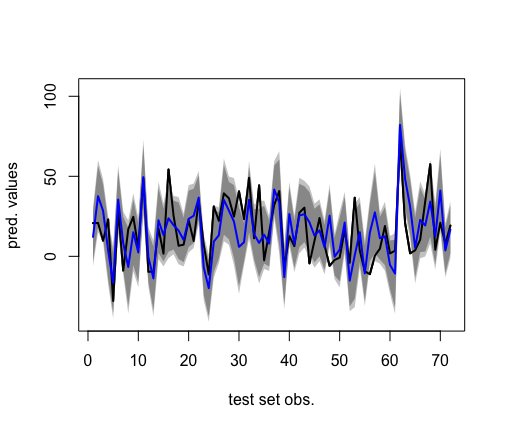
\includegraphics[width=1.064\linewidth, height=0.35\textheight]{gfx/chapter-bayesianrvfl/SLC14_1.png}
        \caption{Out-of-sample predictions and $80$\%, $95$\% confidence intervals for SLC14.1 (with \code{seed = 123})}
        \label{oos_SLC14_1_seed123}
    \end{minipage}%
    \begin{minipage}{0.5\textwidth}
        \centering
        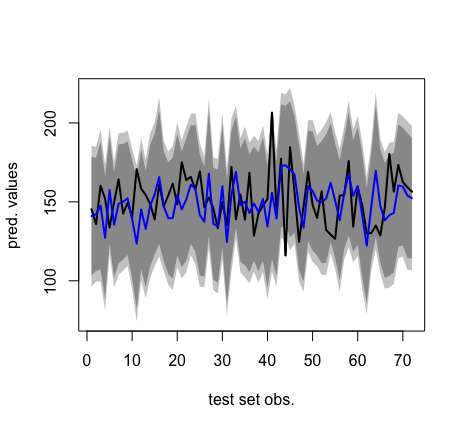
\includegraphics[width=1.064\linewidth, height=0.35\textheight]{gfx/chapter-bayesianrvfl/SLC14_2.png}
        \caption{Out-of-sample predictions and $80$\%, $95$\% confidence intervals for SLC14.2 (with \code{seed = 123})}
        \label{gfx/chapter-bayesianrvfl/oos_SLC14_2_seed123}
    \end{minipage}
\end{figure}
\begin{figure}[!htb]
\centering
    \begin{minipage}{.5\textwidth}
        \centering
        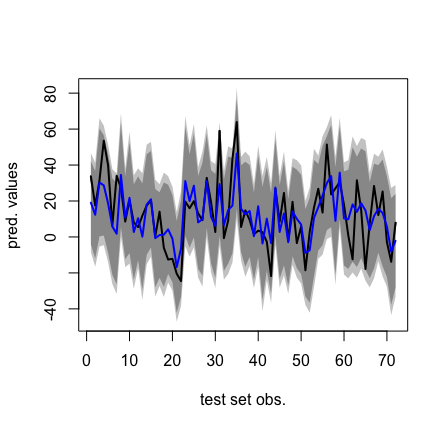
\includegraphics[width=1.064\linewidth, height=0.35\textheight]{gfx/chapter-bayesianrvfl/SLC14_1_seed456.png}
        \caption{Out-of-sample predictions and $80$\%, $95$\% confidence intervals for SLC14.1 (with \code{seed = 456})}
        \label{gfx/chapter-bayesianrvfl/oos_SLC14_1_seed456}
    \end{minipage}%
    \begin{minipage}{0.5\textwidth}
        \centering
        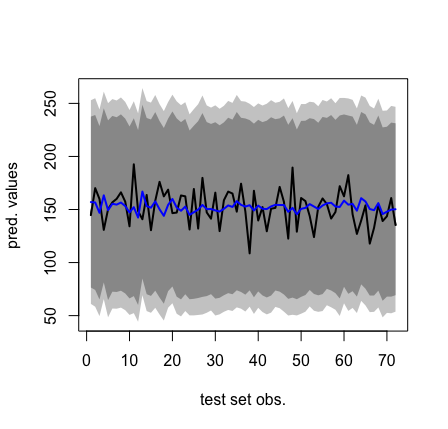
\includegraphics[width=1.064\linewidth, height=0.35\textheight]{gfx/chapter-bayesianrvfl/SLC14_2_seed456.png}
        \caption{Out-of-sample predictions and $80$\%, $95$\% confidence intervals for SLC14.2 (with \code{seed = 456})}
        \label{gfx/chapter-bayesianrvfl/oos_SLC14_2_seed456}
    \end{minipage}
\end{figure}

We observe that the confidence intervals often contain the validation set value, with a few exceptions. The following table \ref{tab:bestparams} contain the \textit{optimal} (based on a grid search) parameters found for each dataset, with a ReLU activation function for the BQRVFL, and the proportions of points of the validation set contained into the $80$\%, $95$\% confidence intervals: 


\begin{table}[!htb]
\begin{center}
% table caption is above the table
\caption{}
\label{tab:bestparams}       % Give a unique label
% For LaTeX tables use
\begin{tabular}{llllll}
\hline\noalign{\smallskip}
Dataset & Number of nodes & $\lambda$ & Prop at 95\% & Prop at 80\% \\
\noalign{\smallskip}\hline\noalign{\smallskip}
   $SLC14_1$ - \code{seed = 123} & 975 & 1.53 & $86.11\%$ & $77.77\%$ \\
   $SLC14_1$ - \code{seed = 456} & -1.047 & -1.024 & $0\%$ & $0\%$ \\
   $SLC14_2$ - \code{seed = 123} & 825 & 20 & $97.22\%$ & $94.44\%$ \\
   $SLC14_2$ - \code{seed = 456} & -1.047 & -1.027 & -1.027 & -1.027 \\
\noalign{\smallskip}\hline
\end{tabular}
\end{center}
\end{table}

\section{Bayesian optimization of black box functions}
\label{sec:bayesopt}

\subsection{Description of the method}

The optimization problem is about finding $\textbf{x}^* \in \AC \subseteq \RR^k$, so that: 

$$
\textbf{x}^* = ArgMin_{\textbf{x} \in \AC} f(\textbf{x})
$$
$f$ is the objective function, whose evaluations are expensive to calculate, and gradients are not necessarily available in closed-form. Methods based on gradient descent, or requiring to evaluate $f$ several times will hence be inefficient for carrying out this task. 

\medskip

Bayesian optimization (cite Mockus et al. (1978) and Jones (2001)) will minimize an alternative, cheaper function called the acquisition function, instead of minimizing $f$ directly. 

\medskip

The acquisition function is based on the uncertainty around the predictions of a surrogate machine learning model, trying to approximate $f$. Here, we consider only two types of acquisition functions. We denote by $\widetilde{f}(\textbf{x}, \theta)$, the prediction obtained with the surrogate model (whose distribution depends on $\theta$) on a point $\textbf{x} \in \AC$: 

\begin{itemize}
\item The \textbf{Upper Confidence Bound} (UCB) acquisition function, (actually a Lower Confidence Bound in the case of minimization). The idea is to minimize: 
$$
a_{UCB}(\textbf{x}) = \mu(\textbf{x}) - \kappa \sigma(\textbf{x})
$$
$\kappa$ is a tuning parameter, designed to balance between exploration and exploitation (more details on this). With $\kappa = 1.96$ for example, this looks like the lower confidence bound of $\widetilde{f}(\textbf{x}, \theta)$, at a risk level of $5$\%, when the surrogate model is $\MN(\mu(\textbf{x}), \sigma(\textbf{x}))$. 

\medskip

\item The \textbf{Expected Improvement} (EI) acquisition function. If $f^*$ is the current minimum value found after a few evaluations of $f$, we would like to maximize the expected improvement of the surrogate model's predictions over $f^*$ :  
$$
a_{EI}(\textbf{x}) = \EE \left[ max(\widetilde{f}(\textbf{x}, \theta) - f^*, 0)\right]
$$
\end{itemize}

\medskip 

The whole optimization process that we use is iterative and is described below, with the total number of iterations denoted as $nb_{iter}$: 

\begin{enumerate}
\item We start with $nb_{init}$ points randomly sampled in $\AC$, for which some evaluations of $f$ have been obtained. With these points, we construct a training data set for the surrogate model:
$$
\DD = \left \lbrace (\textbf{x}_1, f\left(\textbf{x}_1)\right), \ldots,  (\textbf{x}_{nb_{init}}, f(\textbf{x}_{nb_{init}}))\right \rbrace
$$
\item We train the surrogate model on $\DD$, with a fixed parameter $\theta$ for the distribution, and search for the next point to be evaluated for $f$, as: 
$$
\textbf{x}_{next} = ArgMax_{\textbf{x} \in \AC} \: a_{EI}(\textbf{x})
$$ or 
$$
\textbf{x}_{next} = ArgMin_{\textbf{x} \in \AC} \: a_{UCB}(\textbf{x})
$$
If $\textbf{x}_{next}$ is already found in $\DD$, then $\textbf{x}_{next}$ is picked randomly in $\AC$.
\item $\DD$ is enriched with $(\textbf{x}_{next}, f(\textbf{x}_{next}))$ and we return to point $2.$, until the $nb_{iter}$ budget is reached.
\end{enumerate}

Step 2. is done with a gradient based optimization method (cite nlminb PORT routine).

\medskip

For the BQRVFL, we have to choose $\theta$, which, in this specific case, are two parameters: the number of nodes in the hidden layer, and the regularization parameter $\sigma^2$. Ths is done by using Generalized Cross Validation (GCV). More details.  

\medskip

We assume that the Random Forest predictions are Gaussian (you should check this further in the paper of Wager (2014)!). The BQRVFL's posterior distribution is also Gaussian, $\MN(\mu(\textbf{x}), \sigma(\textbf{x}))$. In this case, the acquisition function with  Expected Improvement can be re-written as: 

$$
a_{EI}(\textbf{x}) = \sigma(\textbf{x}) \left( \mu(\textbf{x}) \Phi \left( \gamma(\textbf{x}) \right) +  \Phi^{'} \left( \gamma(\textbf{x}) \right) \right)
$$

\medskip

Where $\Phi$ is the probability distribution function of a $\MN(0, 1)$, and $\Phi^{'}$ is its density function. 

\medskip

This, is to illustrate the model's behaviour on a simple example. A further tuning of the Random Forest hyperparameters, or of the parameter $\kappa$, or a different choice for $nb_{init}$, or activation function for the BQRVFL, would of course lead to different results. For $100$ seeds, and a fixed number of iterations $nb_{iter}$, we rerun the procedure described before, $100$ times. For the BQRVFL, $nb_{iter}$ goes from $5$ to $100$ with steps of $5$, and for the Random Forest with confidence intervals, $nb_{iter} \in \left \lbrace 5, 50, 100 \right \rbrace$. 

\begin{figure}[!htb]
\centering
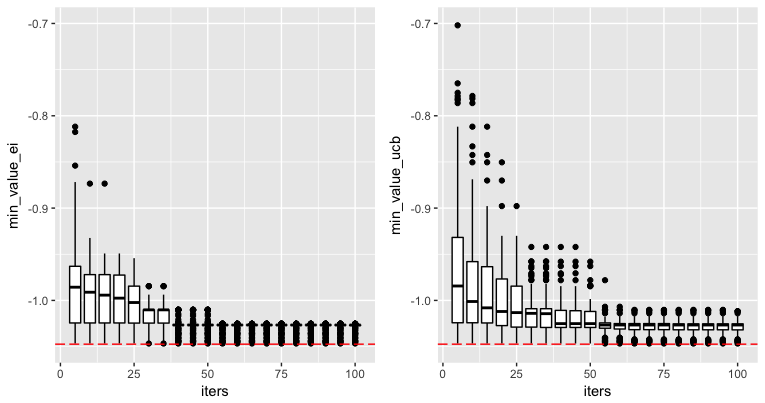
\includegraphics[width=13cm]{gfx/chapter-bayesianrvfl/evol_iter_ei_ucb.png}
\caption{Minimum value for the rescaled Branin function, as a function of the number of iterations with BQRVFL. 
\textbf{Left:} With Expected Improvement (EI) \textbf{Right:} With Upper Confidence Bound (UCB) - BQRVFL}
\label{min_value_dist_bqrvfl}
\end{figure}

\begin{figure}[!htb]
\centering
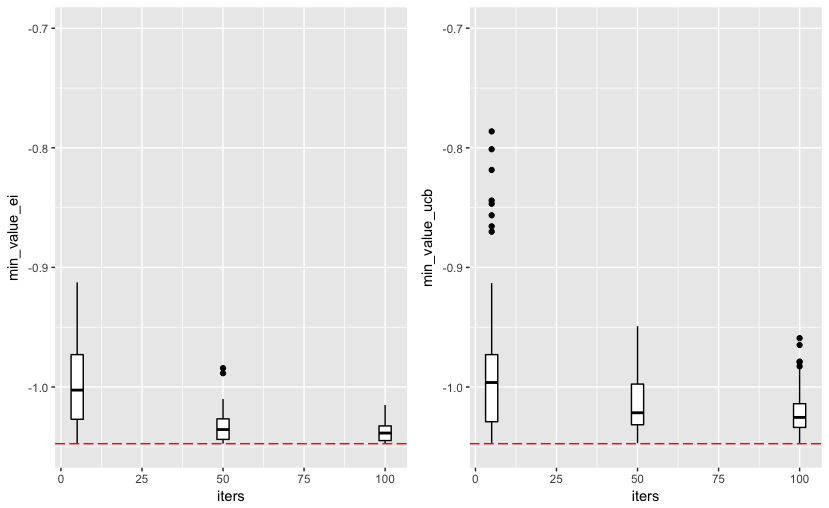
\includegraphics[width=13cm]{gfx/chapter-bayesianrvfl/evol_iter_ei_ucb_rf.png}
\caption{Minimum value for the rescaled Branin function, as a function of the number of iterations. 
\textbf{Left:} With Expected Improvement (EI) \textbf{Right:} With Upper Confidence Bound (UCB) - Random Forest}
\label{min_value_dist_rf}
\end{figure}

\begin{table}[!htb]
\begin{center}
% table caption is above the table
\caption{Summary of minimum values found for the rescaled Branin function, as a function of the number of iterations (with Expected Improvement) with BQRVFL}
\label{tab:min_values_bqrvfl_ei}       % Give a unique label
% For LaTeX tables use
\begin{tabular}{llllllll}
\hline\noalign{\smallskip}
Nb. of iterations & Min & 1st Qrt  & Median & Mean  & 3rd Qrt  & Max & Std. Dev \\
\noalign{\smallskip}\hline\noalign{\smallskip}
  5   & -1.047 & -1.024 & -0.986 & -0.986 & -0.963 & -0.812 & 0.046  \\
  50  & -1.047 & -1.027 & -1.027 & -1.027 & -1.027 & -1.010 & \textbf{0.008} \\
  100 & -1.047 & -1.027 & -1.027 & -1.029 & -1.027 & -1.025 & \textbf{0.006} \\
\noalign{\smallskip}\hline
\end{tabular}
\end{center}
\end{table}

\begin{table}[!htb]
\begin{center}
% table caption is above the table
\caption{Summary of minimum values found for the rescaled Branin function, as a function of the number of iterations (with Upper Confidence Bound) with BQRVFL}
\label{tab:min_values_bqrvfl_ucb}       % Give a unique label
% For LaTeX tables use
\begin{tabular}{llllllll}
\hline\noalign{\smallskip}
Nb. of iterations & Min & 1st Qrt  & Median & Mean  & 3rd Qrt  & Max & Std. Dev \\
\noalign{\smallskip}\hline\noalign{\smallskip}
  5   & -1.047 & -1.024 & -0.984 & -0.963 & -0.932 & -0.702 & 0.079  \\
  50  & -1.047 & -1.029 & -1.025 & -1.020 & -1.012 & -0.958 & 0.017 \\
  100 & -1.047 & -1.032 & -1.027 & -1.028 & -1.025 & -1.012 & 0.008 \\
\noalign{\smallskip}\hline
\end{tabular}
\end{center}
\end{table}

\begin{table}[!htb]
\begin{center}
% table caption is above the table
\caption{Summary of minimum values found for the rescaled Branin function, as a function of the number of iterations (with Expected Improvement) with Random Forest}
\label{tab:min_values_rf_ei}       % Give a unique label
% For LaTeX tables use
\begin{tabular}{llllllll}
\hline\noalign{\smallskip}
Nb. of iterations & Min & 1st Qrt  & Median & Mean  & 3rd Qrt  & Max & Std. Dev \\
\noalign{\smallskip}\hline\noalign{\smallskip}
  5   & -1.047 & -1.027 & \textbf{-1.003} & \textbf{-0.999} & -0.973 & -0.912 & \textbf{0.033} \\
  50  & -1.047 & -1.044 & \textbf{-1.036} & \textbf{-1.033} & -1.027 & -0.984 & 0.012 \\
  100 & -1.047 & -1.045 & \textbf{-1.039} & \textbf{-1.038} & -1.033 & -1.015 & 0.008 \\
\noalign{\smallskip}\hline
\end{tabular}
\end{center}
\end{table}

\begin{table}[!htb]
\begin{center}
% table caption is above the table
\caption{Summary of minimum values found for the rescaled Branin function, as a function of the number of iterations (with Upper Confidence Bound) with Random Forest}
\label{tab:min_values_rf_ucb}       % Give a unique label
% For LaTeX tables use
\begin{tabular}{llllllll}
\hline\noalign{\smallskip}
Nb. of iterations & Min & 1st Qrt  & Median & Mean  & 3rd Qrt  & Max & Std. Dev \\
\noalign{\smallskip}\hline\noalign{\smallskip}
  5   & -1.047 & -1.029 & -0.996 & -0.989 & -0.973 & -0.786 & 0.055 \\
  50  & -1.047 & -1.032 & -1.022 & -1.015 & -0.998 & -0.949 & 0.023 \\
  100 & -1.047 & -1.034 & -1.025 & -1.022 & -1.014 & -0.959 & 0.019 \\
\noalign{\smallskip}\hline
\end{tabular}
\end{center}
\end{table}

Some pretty good results were obtained with the Random Forest for the mean and the median value. But generally with a higher variance on the minimum value obtained than BQRVFL. 

\medskip

Another interesting information obtained through these simulations is the number of times (over $nb_{iter} = 100$ iterations) $\textbf{x}_{next}$ has been picked randomly in $\AC$ at Step 2. (when $\textbf{x}_{next}$ is already in $\DD$). 

\medskip

In table \ref{tab:nb_sims} and figure \ref{nb_is_found_dist}, we observe that on this part, BQRVFL generally performs better. With BQRVFL and Expected Improvement acquisition function for example, the next point to be evaluated is never obtained by simulation of $\textbf{x}_{next} \in \AC$. 

\begin{table}[!htb]
\begin{center}
% table caption is above the table
\caption{Distribution of the number of times a simulation of $\textbf{x}_{next} \in \AC$ has been required at step 2.}
\label{tab:nb_sims}       % Give a unique label
% For LaTeX tables use
\begin{tabular}{llllllll}
\hline\noalign{\smallskip}
Method & Min & 1st Qrt  & Median & Mean  & 3rd Qrt  & Max & Std. Dev \\
\noalign{\smallskip}\hline\noalign{\smallskip}
 BQRVFL with EI  & \textbf{0.00} & \textbf{0.00} & \textbf{0.00}  & \textbf{0.00} & \textbf{0.00} & \textbf{0.00}  & \textbf{0.00} \\
 BQRVFL with UCB & 0.00 & 0.00 & 1.00  & 1.96 & 3.00 & 13.00 & 2.22 \\
 RF with EI      & 0.00 & 2.00 & 3.00  & 3.66 & 5.00 & 9.00 & 1.98 \\
 RF with UCB     & 1.00 & 6.00 & 10.00 & 9.98 & 13.00 & 22.00 & 4.54 \\
\noalign{\smallskip}\hline
\end{tabular}
\end{center}
\end{table}


\begin{figure}[!htb]
\centering
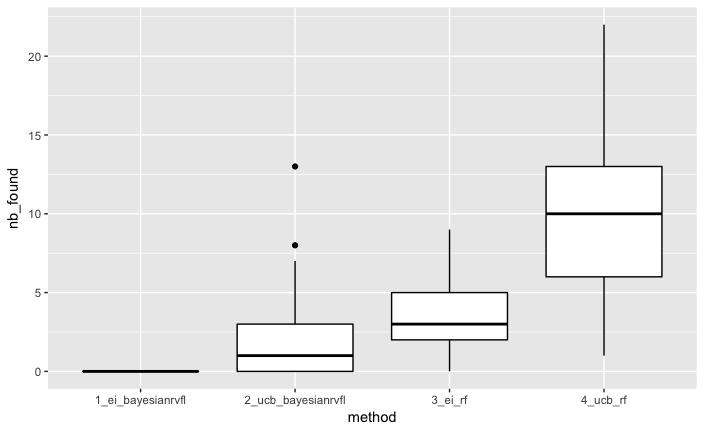
\includegraphics[width=12cm]{gfx/chapter-bayesianrvfl/nb_is_found.png}
\caption{Distribution of the number of times a simulation of $\textbf{x}_{next} \in \AC$ has been required at step 2.}
\label{nb_is_found_dist}
\end{figure}

A good place to apply Bayesian optimization, is to the choice of hyperparameters of machine learning algorithms. The cross-validation function, which is the objective function of the hyperparameters, is indeed expensive to train/predict over the cross-validation resamples.  

\subsection{Example of models based on Dynamic Nelson Siegel and Kernel Regularized Least Squares}

\subsubsection{Description of the models}

In the previous chapters, we introduced the RVFL, the KRLS, and the DNS-KRLS models. Here, we compare all these models by using the Bayesian optimization algorithm described in this chapter.  

\subsubsection{Examples of minimization of the out out-of-sample RMSE}


\begin{table}[!htb]
\begin{center}
% table caption is above the table
\caption{out-of-sample RMSE for models based on the DNS framework}
\label{tab:min_value_ns}       % Give a unique label
% For LaTeX tables use
\begin{tabular}{llllllll}
\hline\noalign{\smallskip}
\textbf{Horizon} & NS-Gaussian & NS-Mat\'ern 3/2  & NS-Mat\'ern 5/2 & NS-RVFL \\
\noalign{\smallskip}\hline\noalign{\smallskip}
 12 & 0.6584  &  0.6590   &   0.6652 & \textbf{0.5483} \\
 18 & 0.8356  &  0.8356   &   0.8356 & \textbf{0.7078} \\
 24 & 1.0130  &  1.0130   &   1.0130 & \textbf{0.8564}\\
 30 & 1.1607  &  1.1607   &   1.1607 & \textbf{1.0289} \\
 36 & 1.2863  &  1.2863   &   1.2863 & \textbf{1.1405} \\
\noalign{\smallskip}\hline
\end{tabular}
\end{center}
\end{table}

\begin{figure}[!htb]
\centering
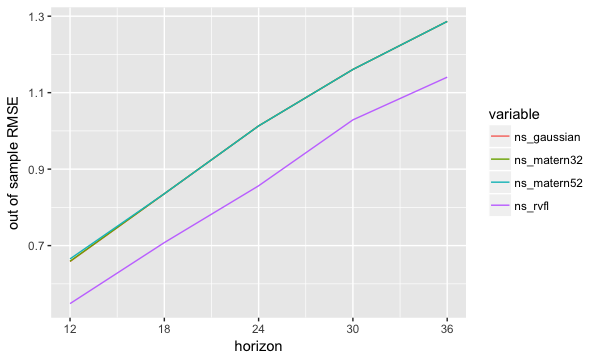
\includegraphics[width=12cm]{gfx/chapter-bayesianrvfl/oos_ns_krls.png}
\caption{out-of-sample RMSE for models based on the DNS framework}
\label{oos_ns_krls}
\end{figure}

\begin{table}[!htb]
\begin{center}
% table caption is above the table
\caption{average out-of-sample RMSE for data-driven KRLS models}
\label{tab:min_value_no_ns}       % Give a unique label
% For LaTeX tables use
\begin{tabular}{llllllll}
\hline\noalign{\smallskip}
\textbf{Horizon} & Gaussian & Mat\'ern 3/2  & Mat\'ern 5/2 & RVFL  \\
\noalign{\smallskip}\hline\noalign{\smallskip}
 12 & 0.6392 & \textbf{0.5168} & 0.5798 & 0.5540 \\
 18 & 0.7466 & \textbf{0.6591} & 0.7394 & 0.7032 \\
 24 & 0.8885 & \textbf{0.7716} & 0.8965 & 0.8191  \\
 30 & 1.0095 & \textbf{0.8844} & 1.0083 & 0.9535  \\
 36 & 1.1544 & \textbf{1.0099} & 1.1396 & 1.0646 \\
 \noalign{\smallskip}\hline
\end{tabular}
\end{center}
\end{table}

\newpage

\begin{figure}[!htb]
\centering
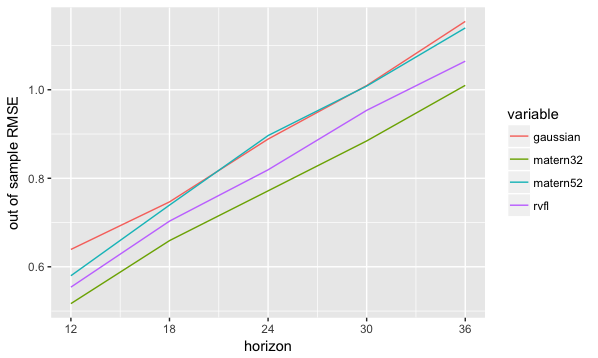
\includegraphics[width=10cm]{gfx/chapter-bayesianrvfl/oos_krls.png}
\caption{average out-of-sample RMSE for data-driven models}
\label{oos_krls}
\end{figure}

Details of the distribution of errors are provided in the appendix (boxplots and summaries). 

We also show how the Mat\'ern 3/2 and the DNS-RVFL are performing over the time, for horizon = $12$ and for horizon = $36$, particularly during the credit/liquidity crunch.



\subsection{Example of ensembles of RVFL}

In this section, we compare the bagging and stacking of RVFL models. As in the previous section, the optimization of the out-of-sample error (the choice of model's hyperparameters) is made by using the BQRVFL as a workhorse for Bayesian optimization. 

\section{Conclusion}

In this chapter, we presented a quasi-randomized functional link neural networks (BQRVFL) model, by linking it to a Bayesian linear regression framework, and obtained formulas for the confidence intervals around its predictions. The BQRVFL model that we constructed is then used as a workhorse for Bayesian optimization, and notably to find \textit{optimal} hyperparameters for all the forecasting models described in the previous chapters.

In general, we observe that the \textit{best} results are obtained in the DNS-KRLS framework by the RVFL (applied to the level, slope and curvature). And in the KRLS framework, the kernel Mat\'ern 3/2 performs the best. This kernel also performs the best overall, in terms of average out-of-sample RMSE. However, it is worth mentioning, as in previous chapters, that the cost of computing the kernel is a quadratic function of the number of input spot rates. 

Figure (\ref{timings}) illustrates this fact very well (see appendix \ref{sec:timings}). It compares the KRLS and RVFL models timings on training and forecasting horizons equal to $12$ months and $36$ months, and respectively $15$, $22$ and $30$ observed time to maturities. The RVFL timings remain relatively stable as the number of time to maturities increase, whereas the KRLS timings increase at a fast pace in the same situation.

\begin{figure}[!htb]
\centering
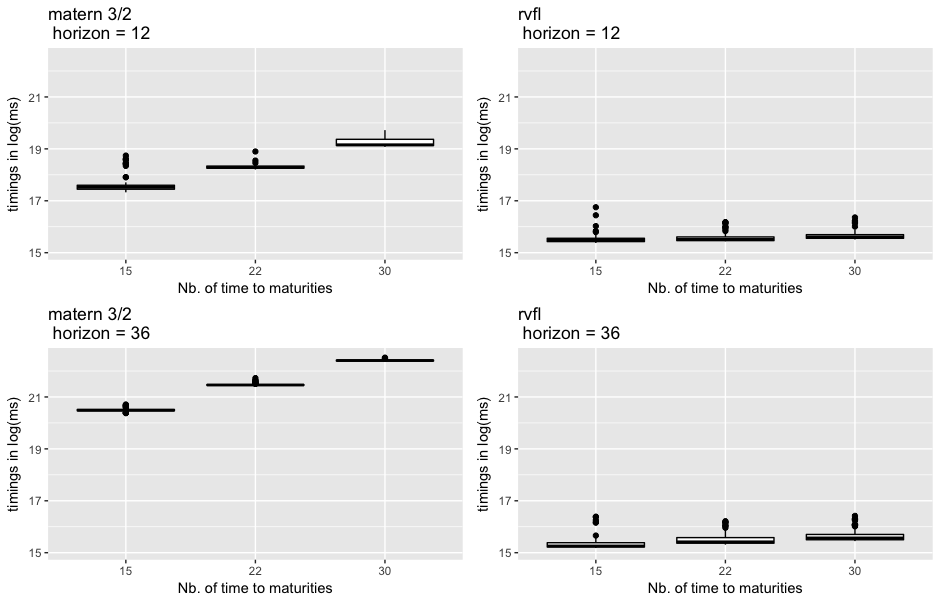
\includegraphics[width=13cm]{gfx/chapter-bayesianrvfl/timings.png}
\caption{timings KRLS vs timings RVFL}
\label{timings}
\end{figure}

When it comes to ensemble learning, we compare bagging, boosting and stacking models. Both.

\newpage

\section{Appendix}

\subsection{Timings in log(ms)}
\label{sec:timings}

\textbf{matern 3/2 - horizon = 12}
\begin{verbatim}
 15              22              30       
 Min.   :17.33   Min.   :18.21   Min.   :19.08  
 1st Qu.:17.45   1st Qu.:18.26   1st Qu.:19.13  
 Median :17.52   Median :18.28   Median :19.16  
 Mean   :17.60   Mean   :18.30   Mean   :19.23  
 3rd Qu.:17.60   3rd Qu.:18.34   3rd Qu.:19.37  
 Max.   :18.74   Max.   :18.90   Max.   :19.72
\end{verbatim}

\textbf{rvfl - horizon = 12}
\begin{verbatim}
15              22              30       
 Min.   :15.37   Min.   :15.44   Min.   :15.51  
 1st Qu.:15.43   1st Qu.:15.47   1st Qu.:15.55  
 Median :15.48   Median :15.51   Median :15.61  
 Mean   :15.53   Mean   :15.58   Mean   :15.66  
 3rd Qu.:15.56   3rd Qu.:15.61   3rd Qu.:15.70  
 Max.   :16.75   Max.   :16.18   Max.   :16.36
\end{verbatim}

\textbf{matern 3/2 - horizon = 36}
\begin{verbatim}
  15              22              30       
 Min.   :20.38   Min.   :21.43   Min.   :22.36  
 1st Qu.:20.47   1st Qu.:21.45   1st Qu.:22.39  
 Median :20.49   Median :21.46   Median :22.40  
 Mean   :20.50   Mean   :21.47   Mean   :22.40  
 3rd Qu.:20.52   3rd Qu.:21.47   3rd Qu.:22.42  
 Max.   :20.71   Max.   :21.73   Max.   :22.52
\end{verbatim}

\textbf{rvfl - horizon = 36}
\begin{verbatim}
15              22              30       
 Min.   :15.18   Min.   :15.31   Min.   :15.45  
 1st Qu.:15.22   1st Qu.:15.37   1st Qu.:15.50  
 Median :15.26   Median :15.42   Median :15.57  
 Mean   :15.35   Mean   :15.51   Mean   :15.65  
 3rd Qu.:15.38   3rd Qu.:15.58   3rd Qu.:15.70  
 Max.   :16.39   Max.   :16.21   Max.   :16.42
\end{verbatim}
